%============================ Project Managenent Document ================================
% define document class
\documentclass[
	a4paper               % paper format
%	,10.5pt               % fontsize
%	,BCOR=18mm            % Binding correction
	,bibliography=totoc   % If enabled add bibliography to TOC
	,listof=totoc         % If enabled add lists to TOC
%	,bilingual
	,monolingual
]{bfhthesis}              % KOMA-script report

\usepackage[
	hidelinks,
	pdfusetitle,
]{hyperref}
\usepackage{tikzducks}
\usepackage{amsmath}
\usepackage{hyperref}

\begin{document}

\frontmatter

\title{Bachelor's Thesis}
\subtitle{Extended BBS?: Management Document}
\author{Joël Gabriel Robles Gasser}
\institution{Bern University of Applied Sciences}
\department{Engineering and Computer Science}
\institute{Computer Science}
\version{0.1}
\advisor{Prof. Dr. Annett Laube \and Prof. Dr. Reto Koenig}
\expert{Dr. Andreas Spichiger}
\degreeprogram{Bachelor of Science in Computer Science}

%----------------  BFH tile page   -----------------------------------------
\maketitle

\addchap{Abstract}
Here an abstract might be placed.


%------------ TABLEOFCONTENTS ----------------
\tableofcontents

%------------ START MAIN PART ----------------
\mainmatter

\chapter{Introduction}
Self-sovereign Identity (SSI)\cite{self-sovereign-identity} is a concept where individuals can control their digital identity and what data is shared with whom.
In the real world physical credentials like an ID or a driver's license are used, which makes selectively disclosing information hard, as there is more information on the credentials as there is needed in one presentation.
If we digitalize these credentials, we create the option for individuals to selectively disclose information. 
Verifiable credentials (VC's)\cite{verifiable-credentials} are a type of digital credentials that can be used to represent physical credentials.
These digital credentials support multiple signing themes, one of which is the BBS Signature scheme (BBS)\cite{bbs-signature-scheme}.
This signature scheme is based on the trust triangle seen in figure \ref{fig:trusttringle}, where there are three involved parties.

\begin{figure}[h]
	\centering
	\includegraphics[width=4cm]{example-image-duck}
	\caption{The trust triangle}
	\label{fig:trusttringle}
\end{figure}

These parties are the issuer, holder and verfier.
The issuer issues the credential, the holder holds the credential and presents it to the verifier, which then verifies the validity of the credential.
This signature scheme supports cryptographic signing as well as cryptographic proof creation, which enables unlinkability.
Unlinkabity is the concept that there is no link between each credential presentation and different verifiers, so no persona about one individual can be created.
BBS also supports selective disclose, to only disclose a subset of the signed messages. With that we have the two most important attributes for this thesis.
In this thesis we assume that the BBS Signature scheme has no flaws, and the promoted unlinkability of the scheme holds in every situation.
We will also only use verifiable-credentials with data integrity, to not only protect the attributes of the credential (like the name, birthdate \dots) but to also protect the meta-data of the verifiable credential.
For the data integrity we will also use the BBS Signature Scheme.
Somehow the credentials need to send between the issuer and holder and between the holder and the verifier.
For this thesis we will only look at the messaging between the holder and the verifier and assume that the VC creation and transportation to the holder is secure.
For the presentation of the credentials there is an extension called a Verifiable-presentation (VP)\cite{verifiable-credentials}.
To present the VP we use OpenID-Connect for Verifiable-Presentations (OIDC4VP)\cite{oidc4vp}.
For OIDC4VP we assume that all communication using the HTTP-protocol is encrypted using TLS.
With this information we now know how to represent a credential in the digital world with VCs, how to secure it against tampering with BBS, to selectively disclose data and use proofs to unlink multiple presentations (also) with BBS, and how to present the credential to verifier using OIDC4VP.
But there are still more things that we can do.
First of we would like to simply the process of a returning customer.
Think about how often you log in into Netflix, either with your email and password or with the cached login token.
It would be very unnecessary to present your credential each time you would like to watch a show, so we would like recognition.
To solve that problem we will look at Pseudonyms\cite{pseudonyms} in chapter \ref{chap:Pseudonyms}.
These Pseudonyms are used for a verifier to recognize already before seen individual.
This extension of the BBS Signature scheme should not break the unlinkability of the BBS proofs as they are only linkable between one verifier and the holder, but will still be analyzed.
Lastly we will look at the problem, where if we need to present two different credentials (like a driver's license and the vehicle registration document), how can we proof that both documents are owned by the same holder.
For that we will make use of link secrets\cite{linksecrets}.
Link Secrets are secret values that only the holder knows.
This value is supplied blinded to the issuer, meaning that is encoded in such a way that the issued cannot find out what the original value is.
For the signer to be able to create a VC containing a blinded value, they would need to use Blind BBS Signatures\cite{bbs-signature-scheme}, which allows signing of such blinded values.
With the blind signatures we also allow individuals to create their own credentials for their own needs, without needing to reveal the content of the credential, by using the ability to blind values.
When a holder then presents two different credentials to a verifier, he can proof that both of those credentials are owned by him by proving the knowledge of the contents of the blinded link secrets.
And with that we have now seen all the extensions that will be thematised in this thesis.
All these extensions we be analyzed for data leakage or for breaking the unlinkability provided by the BBS Signature Scheme.

\chapter{Goals}

\chapter{Recap of BLS12-381, BBS and Pairings}
This chapter contains a quick recap about BBS and BLS12-381.
The Mathematics of these topics are out of scope for this Thesis, so only the top level ideas will be discussed.

\section{BLS12-381}
\begin{figure}[h]
    \centering
	\includegraphics[width=4cm]{example-image-duck}
	\caption{The BLS12-381 curve}
	\label{fig:bls12381}
\end{figure}
The Barreto-Lynn-Scott Curves \cite{pairing-friendly-curves} are a group of pairing friendly curves. 
Specifically the BLS12-381 Curve is used in the BBS Signature Scheme \cite{bbs-signature-scheme}.
The 12 in the name comes from the embedding degree, the 381 is the amount of bits necessary to represent a point on the curve.
This Curve is defined as with the following equation $y^2 = x^3 + 4$, where x and y are coordinates on the Field $F_p$.

\subsection{Field Extensions}
$G_1$ is the largest is the largest prime order subgroup of the BLS curve.
For the Pairings discussed in section \ref{sec:pairing} we need multiple points on curves as inputs.
Besides a point on $G_1$ we also need a point on $G_2$.
This $G_2$ is an Extension of the Field $F_p$ into the Field $F_{p^2}$.
This alters the curve equation a bit to $y^2 = x^3 + 4(u + 1)$ where x and y are no longer coordinates but are polynoms of the second order.
Both $G_1$ and $G_2$ are additive Groups.
For the Pairings we also need a third Group, this time in the Field $F_{p^{12}}$.
This is Group is a multiplicative group called $G_T$ in section \ref{sec:pairing}, where x and y are polynoms of the $12^{th}$ order.
With this we now know all the necessary groups for \ref{sec:bbs}.
The Basepoints (generators) of both $G_1$ and $G_2$ are defined in \cite{pairing-friendly-curves} as follows (Big-endian order encoded as HEX):\newline

\boldmath$G_1$(BP1):\newline
x = 0x17f1d3a73197d7942695638c4fa9ac0fc3688c4f9774b905a14e3a3f171bac586c55e83ff97a1aeffb3af00adb22c6bb
y = 0x08b3f481e3aaa0f1a09e30ed741d8ae4fcf5e095d5d00af600db18cb2c04b3edd03cc744a2888ae40caa232946c5e7e1\newline\newline
\boldmath$G_2$(BP2):\newline
$x_O$ = 0x024aa2b2f08f0a91260805272dc51051c6e47ad4fa403b02b4510b647ae3d1770bac0326a805bbefd48056c8c121bdb8
$x_1$ = 0x13e02b6052719f607dacd3a088274f65596bd0d09920b61ab5da61bbdc7f5049334cf11213945d57e5ac7d055d042b7e
$y_O$ = 0x0ce5d527727d6e118cc9cdc6da2e351aadfd9baa8cbdd3a76d429a695160d12c923ac9cc3baca289e193548608b82801
$y_1$ = 0x0606c4a02ea734cc32acd2b02bc28b99cb3e287e85a763af267492ab572e99ab3f370d275cec1da1aaa9075ff05f79be

\section{BBS}
\label{sec:bbs}
\begin{figure}[h]
    \centering
	\includegraphics[width=4cm]{example-image-duck}
	\caption{The Actors of BBS and their connection}
	\label{fig:bbstriangle}
\end{figure}
The BBS Signature Scheme \cite{bbs-signature-scheme} is a multi-message signature scheme with support for selective disclosure and proof of knowledge of the signature, thus proving unlinkability between different verfiers. 
Figure \ref{fig:bbstriangle} shows the flows between the different actors.
For this thesis we define following names for the actors:
\begin{itemize}
	\item Issuer - Issues a signature on a set of messages
	\item Holder - Holds the set of messages as well as the signature. Also generates the Proof for the verifier.
	\item Verifier - Gets the disclosed messages as well as the proof, which he then verifies
\end{itemize}
For the key generation a random scalar \textbf{SK} and the Base Point of $G_2$ are needed.
Thus the public key (calculated as $SK*BP2$) results in Point on $G_2$.
This allows for all other calculations (like the signature or the proof) to be done in $G_1$ which in turn makes the algorithm more efficient.


\section{Pairings}
\label{sec:pairing}
For the verification of the BBS signature and proof Pairing-functions are used. The most important part of these functions are their billiniarity i.e.,\newline
\begin{equation}
		e(A, B + B') = e(A, B)e(A, B') \text{and} e(a * A, b * B) = e(A, B)^{ab}
\end{equation}

With these characteristics we can understand the equations for verifying the signature and proof.\newline

\textbf{Example 1. BBS Signature verification}
\begin{equation}
	\begin{split}
		Identity_{GT} & = e(A, W + BP2 * e) * e(B, -BP2) \\
		& = e(A, BP2 * e)e(A, W)e(B, BP2)^{-1} \\
		& = e(A, BP2)^ee(A, SK * BP2)e(B, BP2)^{-1} \\
		& = e(A, BP2)^ee(A, BP2)^{SK}e(B, BP2)^{-1} \\
		& = e(A, BP2)^{e + SK}e(B, BP2)^{-1} \\
		& = e(B * \frac{1}{sk * e}, BP2)^{e + SK}e(B, BP2)^{-1} \\
		& = e(B, BP2)^{\frac{e + SK}{e + SK}}e(B, BP2)^{-1} \\
		& = e(B, BP2)^1e(B, BP2)^{-1} \\
		& = e(B, BP2)^0 \\
		& = 1
	\end{split}
\end{equation}

\chapter{Use Cases}
For this Thesis we will use a small collection of use cases to demonstrate how BBS should work in conjunction with extensions (like VC's, Link Secrets etc.).

\section{Simply buying a train and mobile subscription}
Lets assume you want to go and buy a train subscription.
Once at the counter, the employee ask you for your ID card, to verify your identity and to get the required data for the subscription.
Now the employee should only need to check if the ID is valid, if the photo on it matches you, something to link your subscription to you (your name is used for that most of the time) and maybe he also needs your birthday for an age specific discount.
By handing out your ID, you lose the ability to selectively disclose information about yourself, and with that you lose your anonymity.


\begin{figure}[h]
	\begin{minipage}{0.28\textwidth}
		\textbf{Client}\newline\newline
		
\begin{tikzpicture}
			\duck[graduate]
		\end{tikzpicture}
	\end{minipage}\hfill
	\begin{minipage}{0.28\textwidth}
		$$\underrightarrow{\includegraphics[width=30mm]{./img/ID.jpg}}$$
		$$\overleftarrow{\includegraphics[width=30mm]{./img/Swisspass.jpeg}}$$
	\end{minipage}\hfill
	\begin{minipage}{0.28\textwidth}
		\textbf{SBB}\newline\newline
		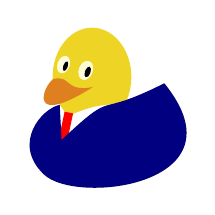
\begin{tikzpicture}
			\duck[tshirt, jacket=blue!50!black, tie=red]
		\end{tikzpicture}
	\end{minipage}
	\caption{Buying a train subscription}
	\label{fig:trainsub}
\end{figure}

Now you also need a mobile subscription. You go to your next Swiss Post office.

\begin{figure}[h]
	\begin{minipage}{0.28\textwidth}
		\textbf{Client}\newline\newline
		
\begin{tikzpicture}
			\duck[graduate]
		\end{tikzpicture}
	\end{minipage}\hfill

	\begin{minipage}{0.28\textwidth}
		$$\underrightarrow{\includegraphics[width=30mm]{./img/ID.jpg}}$$
		$$\overleftarrow{\includegraphics[width=30mm]{example-image-duck}}$$
	\end{minipage}\hfill

	\begin{minipage}{0.28\textwidth}
		\textbf{Swiss Post}\newline\newline
		
\begin{tikzpicture}
			\duck[tshirt, jacket=yellow!50!orange, tie=black]
		\end{tikzpicture}
	\end{minipage}
	
	\caption{Buying a mobile subscription}
	\label{fig:mobilesub}
\end{figure}

Here, the employee makes the same checks as the SBB employee to see if you are who you say you are.
And again, by handing out your ID, you lose the ability to selectively disclose information about yourself.

\begin{figure}
	\includegraphics[width=30mm]{example-image-duck}
\end{figure}

Now lets say but verifiers collude. As they have the same information about you, they link it back to you and create a profile about.
In \autoref{chap:bbsex} we will see how we can use BBS to restore unlinkability and more.
	



 
	





\chapter{Extensions of BBS}
\label{chap:bbsex}

\section{BBS with VC's}
The BBS signatures and proofs as well as the messages need to be transported somehow.
For this Thesis we chose Verifiable credentials \cite{verifiable-credentials} as the representation of these attributes.
But what are VC's? \newline
Verifiable credentials are JSON-LD data models, designed to represent different types of digital credentials.
The Idea, is to be able to translate physical credentials, like an ID or a driver's license, into the digital world.
In this Thesis we will only look at a small part of the standard, just enough that we can use it together with BBS.

\subsection{Prepare VC's for BBS}


\section{BBS with Pseudonyms}
\label{chap:Pseudonyms}

\section{BBS with Link Secrets}
\label{chap:linksecrets}

\section{BBS with Blind Signatures}
\label{chap:blindsignatures}




\appendix

\chapter{First appendix Chapter}



\bibliographystyle{plain}
\bibliography{refs}

\end{document}
